\documentclass[12pt,english]{article}
\usepackage{geometry}[margin=2]
\usepackage{blindtext}
\usepackage{enumerate}
\usepackage{parskip} 
\usepackage{siunitx}
\usepackage{amsmath}
\usepackage{amsfonts}
\usepackage{amssymb}
\usepackage{hyperref}
\usepackage{listings}
\usepackage{inconsolata}
\usepackage{parskip}
\usepackage{graphicx}
\usepackage{wrapfig}
\graphicspath{./images}
\author{
    Cole Johnson: \texttt{cole.johnson.@student.nmt.edu}
    \\ 
    John Runyon: \texttt{john.runyon@student.nmt.edu}
}
\title{
    CSE441: Project Proposal\\
    \large{Cryptanalysis of Hash Functions}
}
\begin{document}
\maketitle
\section*{Introduction and Outline of Project}
\subsection{The Basics of Hash Functions}
Hashing, as an overall process, is a function that maps
plaintext data of any length into a fixed-length ciphertext
output--often called a digest. Hash functions, unlike encryption,
destroy information encoded in the plaintext, which means
the function is one-way and cannot be reversed to obtain
the plaintext again.

\begin{wrapfigure}{r}{0.5\textwidth}
    \begin{center}
      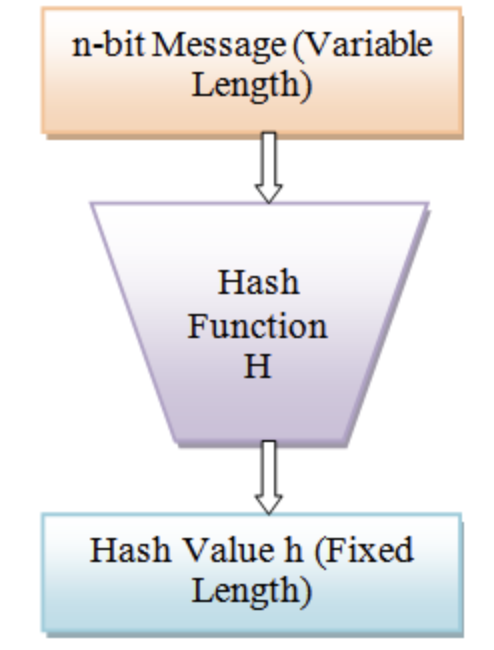
\includegraphics[clip=true,height=5cm, width=0.3\textwidth]{images/hash_function.png}
    \end{center}
    \caption{Basic diagram of a hash function}
  \end{wrapfigure}

Hash functions are a widely used type of cryptographic algorithm.
They can be used for a variety of purposes, such as
data integrity verification, password storage, and digital
fingerprint/signatures, and data indexing (often called hash-tables).
Since hash functions serve vital purposes in modern cryptography
and computer science, knowing the important mathematical properties
of a hash function (and how these can be implemented in programs)
is critical to understanding their function. \\ 

Once the function and real-world implementation of a hash function is understood, it becomes clear why certain mathematical properties, such as determinism, pre-image resistance, and collision resistance are crucial. These properties ensure that hash functions can efficiently convert data of any size into a fixed-length output while preventing malicious actors from reversing or tampering with the data. The fixed length output is a major factor of any hashing algorithm - meaning that a user can input one character or one-hundred characters, and still receive a 256-bit hash as is the case with SHA-256.

\subsection{Outline of Project}
Here is the sections of the project, along with a small description 
of what each of the sections will cover:
\begin{enumerate}[{\bf (a.)}]
    \item Introduction to Hash Functions
    \begin{enumerate}
        \item Basics of Hash Functions (including code examples, and diagrams)
        \item Legacy/Classic and Modern Hash Functions and their Applications
        \item Hash Functions Examples (MD5, SHA-256, Tornado)
    \end{enumerate} 
    \item Properties of Hash Functions
    \begin{enumerate}
        \item One-way Function (Pre-Image Resistance)
        \item Target Collision Resistance (2nd Pre-Image Resistance)
        \item Deterministic
        \item Avalanche Effect
        \item Computational Speed
    \end{enumerate}
    \item Cryptanalysis and Attacks on Cryptographic Hash Functions
    \begin{enumerate}
        \item Brute-Force Attacks
        \item One-way Function Inversion
        \item 2nd Pre-Image Resistance Attack
        \item Collision Attack
    \end{enumerate}
\end{enumerate}
\subsection{Experimentation}
For our experimentation our group is wanting to look into the varying overhead required by different crytographic algorithms such as MD5, SHA-1, and SHA-256. This could include using local machines for testing and online research to find and compare the available data on the performance of different hash functions in terms of speed and the use of resources. Our reasoning and conclusion of this experimentation would result in a conversation on the trade-offs between security and speed and the different use cases for each.
\subsection{Conclusion}
Our project will explore the process of cryptoanalysis of various hash functions as mentioned above - aiming to research not only the practical, but the theoretical as well. By analyzing the performance, and security of varying hash functions we aim to better understand the trade-offs that exists amongst these algorithms. Our testing of these functions will give us a real world example and the implications especially in terms of the overhead involved. \\

Hash functions are critical to the modern internet and computer infrastructure, so understanding their uses is not only important, but critical for security and ensuring data integrity. We look forward to evaluating our experiments and possibly offering insight on the current state of hashing in the space of cryptography.
\end{document}
